To start the bridge between the world of Algebra as we know it and geometry, there must be an established way to discuss geometry algebreically. This is where the concepts of affine spaces comes in.  

This concept allows the analysor to view the geometry algebreically. However, this is not the endgoal, but an analytic step between geometry and the more powerful algebreic tools that we want to apply to geometry. 

Affine maps as generalizations of linear maps. \cite{gallier2025affine}

Vector spaces being limiting since origin is given special consideration, bad \cite{gallier2025affine}

Frame invariance.

\subsubsection{Affine Spaces}

\begin{definition}
    An \textit{affine space} is either the empty set, or a triple $<E, \vec{E}, +>$. $E$ is a nonempty set of points while $\vec{E}$ is a vector space (of translations). The action $+$ is an operation on both $E$ and $\vec{E}$ defined as follows: $+: E \times \vec{E} \rightarrow E$. The following axioms are assumed for affine space:
    \begin{enumerate}[label=A\arabic*]
        \item $a + 0 = a$ for every $a \in E$.
        \item $(a + u) + v = a + (u + v)$ for every $a \in E$ and every $u,v \in \vec{E}$.
        \item For any two points $a,b \in E$, there is a unique $u \in \vec{E}$ such that $a + u = b$
    \end{enumerate}
\end{definition}

\begin{figure}[ht]
    \centering
    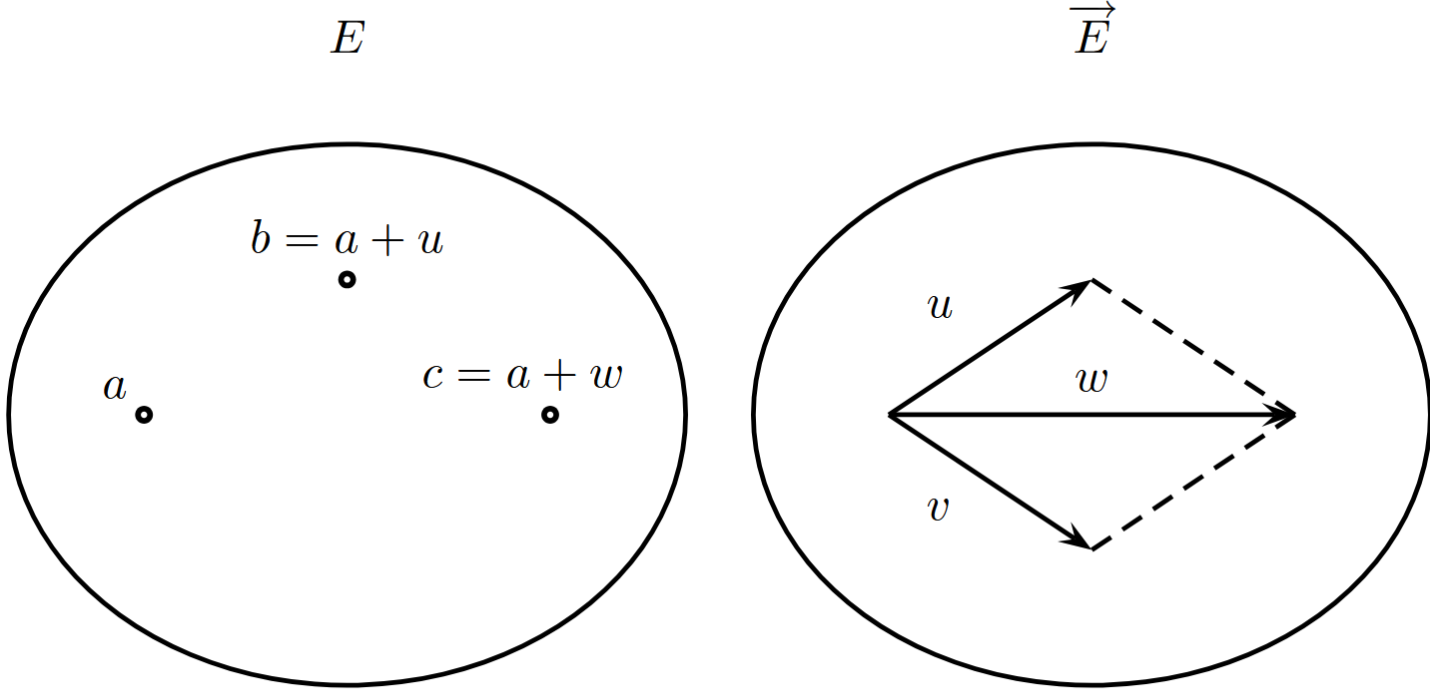
\includegraphics[width = \textwidth]{figures/AffineSpace.png}
    \label{fig:affineSpace}
    \caption{Intuiative understanding of affine space \cite{gallier2025affine}}
\end{figure}
\subsubsection{Affine Varieties}
